\documentclass[10pt, a4paper]{article}

% \usepackage[mathdisplays=normal]{savetrees}

% Core packages for better typography
\usepackage[utf8]{inputenc}
\usepackage[T1]{fontenc}
\usepackage{lmodern}
% \usepackage{newtxtext,newtxmath}
\usepackage{latexsym,amsfonts,amssymb,amsthm,amsmath}
\usepackage{mathtools}
\usepackage{textcomp}
\usepackage{microtype}
\usepackage{setspace}
\usepackage{siunitx}
\DeclareSIUnit{\um}{\ensuremath{\mu}\mathrm{m}}
% \onehalfspacing

% Math packages with better formatting

% Graphics and figures
\usepackage{tikz}
\usetikzlibrary{angles,quotes}
\usepackage{pgfplots}
\pgfplotsset{compat=newest}
\usepackage{graphicx}
\graphicspath{{../data/}}

% Better table formatting
\usepackage{booktabs}
\usepackage{array}
\usepackage{multirow}

% Force figures to stay in their sections
\usepackage[section]{placeins}
\makeatletter
\AtBeginDocument{%
  \expandafter\renewcommand\expandafter\subsection\expandafter{%
    \expandafter\@fb@secFB\subsection
  }%
}
\makeatother

% Code listing formatting
\usepackage{listings}
\usepackage{xcolor}
\definecolor{codegreen}{rgb}{0,0.6,0}
\definecolor{codegray}{rgb}{0.5,0.5,0.5}
\definecolor{codepurple}{rgb}{0.58,0,0.82}
\definecolor{backcolour}{rgb}{0.95,0.95,0.92}
\lstdefinestyle{mystyle}{
  backgroundcolor=\color{backcolour},   
  commentstyle=\color{codegreen},
  keywordstyle=\color{blue},
  numberstyle=\tiny\color{codegray},
  stringstyle=\color{codepurple},
  basicstyle=\ttfamily\footnotesize,
  breakatwhitespace=false,         
  breaklines=true,                 
  captionpos=b,                    
  keepspaces=true,                 
  showspaces=false,                
  showstringspaces=false,
  showtabs=false,                  
  tabsize=2
}
\lstset{style=mystyle}

% References and hyperlinks
\usepackage{pdfpages}
\usepackage[colorlinks=true, linkcolor=blue, citecolor=blue]{hyperref}
\usepackage{caption}
\usepackage{subcaption}
\usepackage{csquotes}
\usepackage[notes, backend=bibtex]{biblatex-chicago}
\addbibresource{refs.bib}



% Custom theorem environments
\newtheorem{theorem}{Theorem}[section]
\newtheorem{lemma}[theorem]{Lemma}
\newtheorem{proposition}[theorem]{Proposition}
\newtheorem{corollary}[theorem]{Corollary}
\newtheorem{definition}{Definition}[section]
\newtheorem{example}{Example}[section]

\title{\Large \bfseries SB4: Integrated Photonics\\[0.5em] \large Final Report}
\author{Lucas Ng\thanks{ln373@cam.ac.uk}}
\date{13th June 2025}

\begin{document}
\maketitle

\section{Introduction}

In the first interim report, we performed modal analysis on a symmetric planar waveguide
of several core and cladding materials, with further investigation into the effects of waveguide geometry and modal excitation wavelength on the modal properties,
including the effective index, group index, birefringence, and dispersion characteristics.

The second interim report recognised that waveguides do not exist in isolation,
and presented the coupled mode theory as a framework for understanding the power transfer across coupled waveguides,
with a derivation via considering the coupled mode propagation matrix,
\[
\mathbf{M} = \begin{pmatrix}
\beta & \kappa \\
\kappa & \beta
\end{pmatrix},
\]
to be the infinitessimal generator matrix that generates the modal evolution transition matrix as 
a one-parameter subgroup of the Lie group \(GL(2, \mathbb{C})\)
via the exponential map \(-jzM\mapsto e^{-jzM}\) (where \(z\) is the propagation distance along the waveguide)
that acts on an element of the Lie algebra \(\mathfrak{gl}(2, \mathbb{C})\).
This formalism demonstrated how the intrinsic structure of \(M\) gives rise to the modal properties of the coupled waveguide:
the symmetry of the matrix \(M\) corresponds to reciprocal coupling,
while real-valued \(\beta\) and \(\kappa\) encodes the conservation of power in the coupled waveguide,
since in this instance, \(-jzM\) is Hermitian, and thus the image of the exponential map is unitary.

Likewise, this current, final report, ascends to the next level of abstraction,
\textit{\'a la mise en abyme},
considering the whole structure of a S-bend directional coupler in its entirety.
At this level, the previous theoretical frameworks serve purely as approximation,
and we must account for bending losses, asymmetric couplers, and other practical and interesting considerations.
This being analytically intractable, Lumerical's FDTD software\autocite{lumerical_fdtd} was utilised to simulate the directional coupler.

\section{Simulation setup}

The geometry of our directional coupler is the traditional doubly-symmetric S-bend design,
with a parallel coupling length connected in each waveguide to its input and output ports by S-bends.
Each port is extended by a straight waveguide which extends through to \SI{1}{\um} outside the FDTD simulation region,
which is otherwise internally padded on all sides by \SI{2.5}{\um} of perfectly matched layer (PML) boundary conditions.
The input port of the upper waveguide is excited by a modal source at the wavelength of interest.

This form of the directional coupler is, by way of metaphor, structured as an aubade.
Figure~\ref{fig:s_bend_coupler} shows how the geometry is parameterised by the widths of each waveguide (which may be varied independently),
the separation gap between the two waveguides, the length of the coupling region,
and the wavelength of the modal source.
The waveguide material is silicon with a cladding of silicon dioxide,
with wavelength-dependent refractive indices taken from the \texttt{Si (Silicon) - Palik}
and \texttt{SiO2 (Glass) - Palik} entries of the Lumerical material database respectively.
The waveguide depth into the plane is \SI{220}{\nm} for both waveguides,
the ports on each end are separated by \SI{10}{\um} in the horizontal direction,
and the poles of the S-bends are placed at \([(0,0), (\pm 5, 0), (\pm 5, \mp 5), (\pm 5, \mp 5)]\)\,\unit{\um}.
The TE\textsubscript{0} mode is launched at the input port.

% TODO: Add a figure of the S-bend directional coupler geometry.
\begin{figure}[h!]
  \centering
  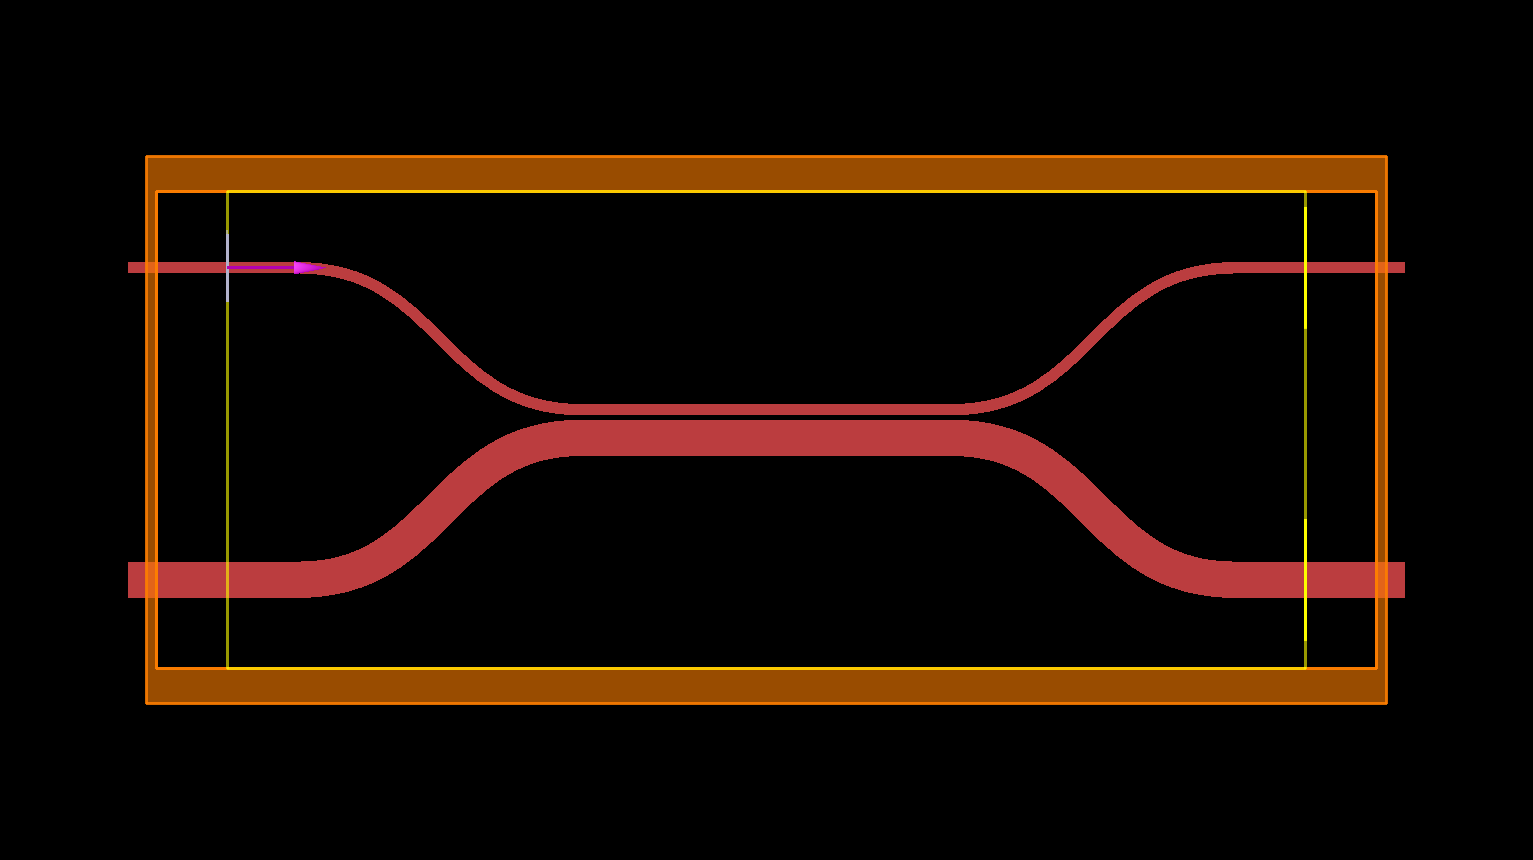
\includegraphics[width=0.8\textwidth]{task3/views/wg1_width=0.4_wg2_width=1.28_separation=0.15_coupling_length=13.0.png}
  \caption{Schematic of the S-bend directional coupler geometry
  with parameters \(w_1=\SI{400}{\nm}\), \(w_2=\SI{1280}{\nm}\), \(\text{separation}=\SI{150}{\nm}\), and \(L=\SI{13.0}{\um}\).}
  \label{fig:s_bend_coupler}
\end{figure}

\section{Results}

\subsection{TE\textsubscript{0}-TE\textsubscript{0} coupling}

For equal waveguide widths, it is quite straightforward to achieve arbitrary TE\textsubscript{0}-TE\textsubscript{0} power transfer between the two coupled waveguides.
With TE\textsubscript{0} launched at the input port of the upper waveguide, a co-located waveguide symmetrised across the separation gap supports TE\textsubscript{0} at the same effective index
(subject to fabrication tolerances),
and thus the TE\textsubscript{0} mode is coupled to the TE\textsubscript{0} mode of the lower waveguide.

Other modes have a large phase mismatch \(\Delta\beta=k_0\Delta n_\text{eff}\gg 1\) with respect to TE\textsubscript{0},
and hence cross-mode leakage has a negligible modal power beating amplitude of

\[A\propto\frac{\kappa^2}{\kappa^2+{(\frac{\Delta\beta}{2})}^2}\approx{\left(\frac{2\kappa}{\Delta\beta}\right)}^2\to 0.\]

Moreover, by selecting the waveguide width to be sufficiently small, higher order modes can be suppressed,
as they are not supported by the waveguide geometry.

The proportion of the power transferred to the lower waveguide is then a function of the coupling length \(L\),
\[
P\propto\sin^2\left(\frac{\kappa L}{2}\right),
\]
where \(\kappa\) is the coupling coefficient, which is a function of the waveguide geometry and the wavelength of the modal source.

\paragraph{Power transfer as a function of coupling length}
Figure~\ref{fig:coupling_length} shows the power transfer as a function of the coupling length \(L\) for a fixed waveguide width of \SI{500}{\nm} and separation gap of \SI{150}{\nm},
with the TE\textsubscript{0} mode launched at a wavelength of \SI{1550}{\nm} from the input port of the upper waveguide.
The coupled mode theory predicts sinusoidal power beating, with half-power transfer to occur at a minimum coupling length of \(L_{3\text{db}}=\frac{\pi}{4\kappa}\),
and for total power transfer to occur at a minimum coupling length \(L_c=\frac{\pi}{2\kappa}\).
Indeed, we observe \(\hat{L}_{3\text{db}}\approx\SI{10}{\um}\) and \(\hat{L}_c\approx\SI{21}{\um}\) in the simulation results. 
This implies a coupling coefficient of \(\hat{\kappa}\approx\SI{0.4}{\um^{-1}}\).

\begin{figure}[h!]
  \centering
  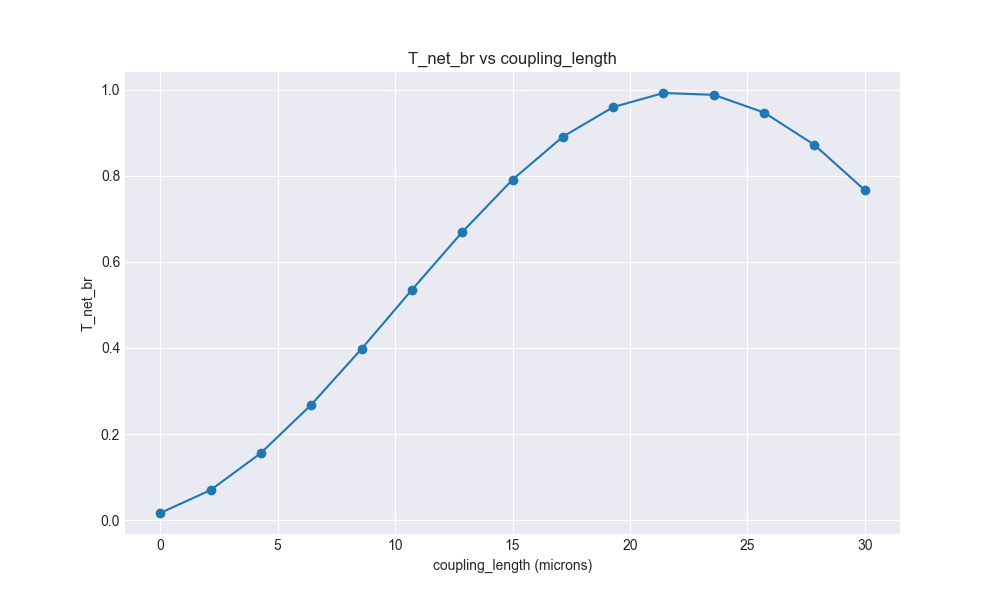
\includegraphics[width=0.8\textwidth]{task3/sweep_plots/sweep_idx_0_sweep__coupling_length=0_30_15_T_net_br_line.png}
  \caption{Cross-power transfer fraction at the coupled output port as a function of coupling length \(L\) for a fixed waveguide width of \SI{500}{\nm} and separation gap of \SI{150}{\nm} under input port TE\textsubscript{0} mode excitation at \SI{1550}{\nm}.}
  \label{fig:coupling_length}
\end{figure}


\paragraph{Half-power transfer}
Figure~\ref{fig:eq_power_distribution} shows the power intensity distribution across the waveguide plane
for the half-power simulation at \(\hat{L}_{3\text{db}}\approx\SI{10}{\um}\).
The TE\textsubscript{0} mode monitor registers a power transfer fraction of
\(0.5056\) while the lower waveguide TE\textsubscript{0} mode monitor registers a power transfer fraction of
\(0.4895\). This implies some power loss, but higher-order mode monitors
show that either the mode is not supported, or that the power transfer fraction is negligible.

\begin{figure}[h!]
  \centering
  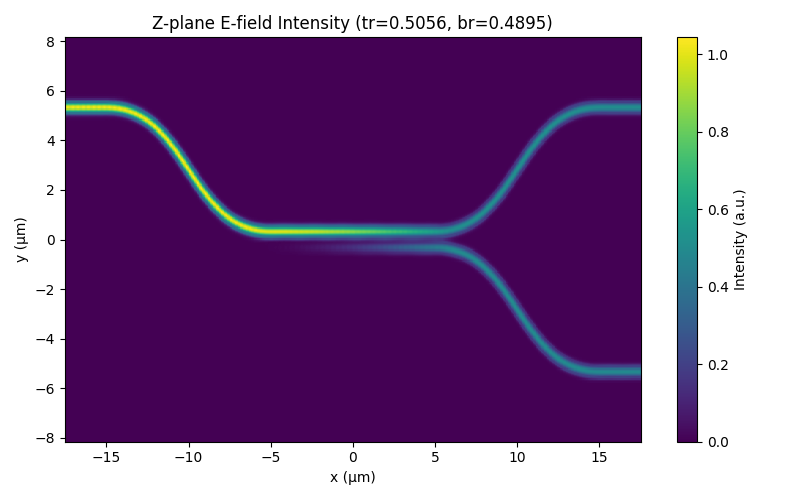
\includegraphics[width=0.8\textwidth]{task3/sim_1742_110625/z_plane_intensity.png}
  \caption{Power intensity distribution across the waveguide plane at the half-power coupling length \(\hat{L}_{3\text{db}}\approx\SI{10}{\um}\) for a fixed waveguide width of \SI{500}{\nm} and separation gap of \SI{150}{\nm} under input port TE\textsubscript{0} mode excitation at \SI{1550}{\nm}.}
  \label{fig:eq_power_distribution}
\end{figure}

\paragraph{Total power transfer}
Figure~\ref{fig:max_power_distribution} shows the power intensity distribution across the waveguide plane
for the total power transfer simulation at \(\hat{L}_c\approx\SI{21}{\um}\).
With cross-mode power transfer to the lower waveguide TE\textsubscript{0} mode monitor registering a power transfer fraction of
\(0.9920\), we can conclude that the upper TE\textsubscript{0} mode is indeed coupled strongly to the lower waveguide TE\textsubscript{0} mode.
This latter parameter set gives us an optimised directional coupler operating at \(\lambda=\SI{1550}{\nm}\).

It should be noted that such a small separation gap utilised above is the minimum of what is achievable in practice,
and in the next section we will explore the effect of varying the separation gap on the power transfer fraction.

\begin{figure}[h!]
  \centering
  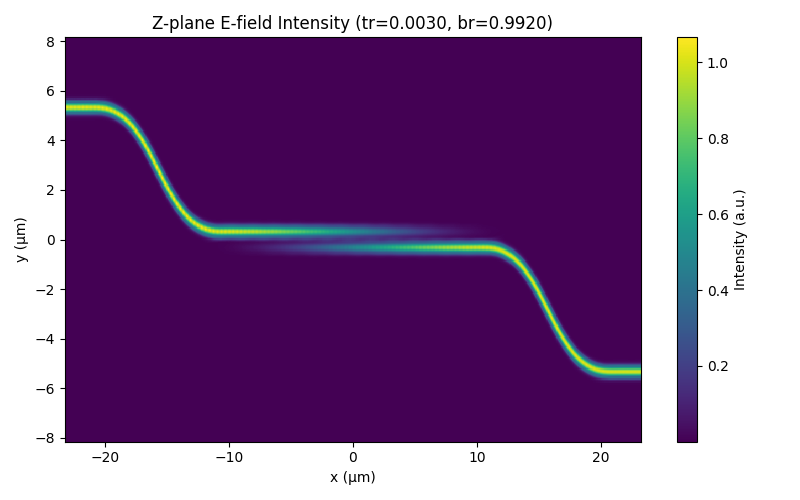
\includegraphics[width=0.8\textwidth]{task3/sim_2318_110625/z_plane_intensity.png}
  \caption{Power intensity distribution across the waveguide plane at the total power transfer coupling length \(\hat{L}_c\approx\SI{21}{\um}\) for a fixed waveguide width of \SI{500}{\nm} and separation gap of \SI{150}{\nm} under input port TE\textsubscript{0} mode excitation at \SI{1550}{\nm}.}
  \label{fig:max_power_distribution}
\end{figure}

\paragraph{Optimising for a shorter wavelength}
To additionally optimise a directional coupler for a shorter wavelength \(\lambda=\SI{1310}{\nm}\), we could repeat the above procedure with the same fixed waveguide width of \SI{500}{\nm} and separation gap of \SI{150}{\nm}.
However, a shorter wavelength requires a larger coupling length to achieve the same fraction of power transfer.
% TODO: add the maths for why

Figure~\ref{fig:coupling_length_1310} shows the power transfer as a function of the coupling length \(L\) for a fixed waveguide width of \SI{500}{\nm} and separation gap of \SI{150}{\nm} over the same swept range as before,
and within this range, we cannot even achieve half-power transfer,
let alone total power transfer. It seems that either we need to have a very large coupling length,
or to modify the waveguide geometry.

\begin{figure}[h!]
  \centering
  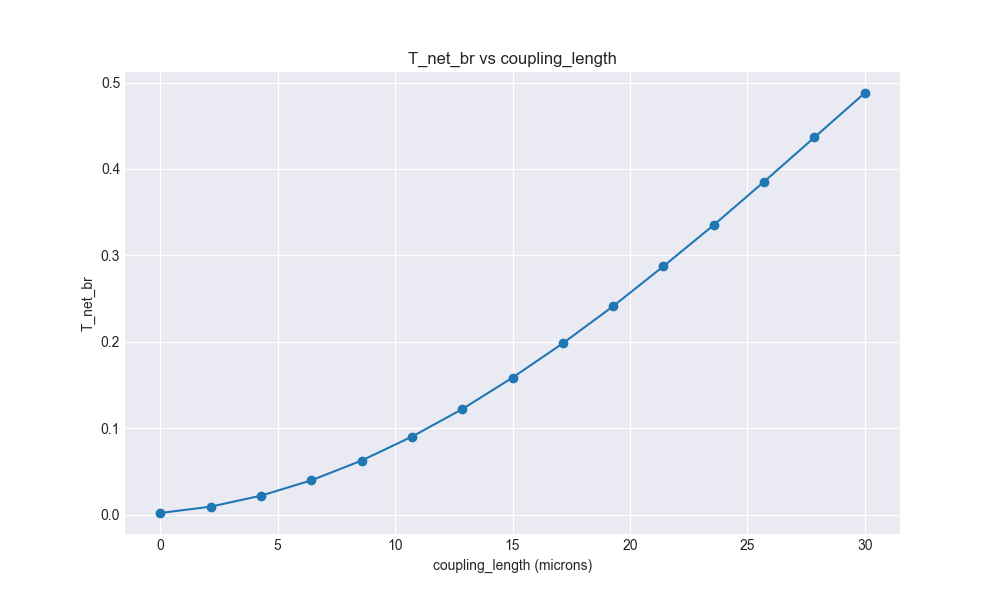
\includegraphics[width=0.8\textwidth]{task3/sweep_plots/sweep_idx_1_sweep__coupling_length=0_30_15,_center_wavelength=1.31_T_net_br_line.png}
  \caption{Cross-power transfer fraction at the coupled output port as a function of coupling length \(L\) for a fixed waveguide width of \SI{500}{\nm} and separation gap of \SI{150}{\nm} under input port TE\textsubscript{0} mode excitation at \SI{1310}{\nm}.}
  \label{fig:coupling_length_1310}
\end{figure}

\paragraph{Reducing the coupling length}
Assuming fabrication tolerances are not a concern
and we do not require the dimensions of the directional coupler to match other components in the photonic circuit, like cascaded couplers or integrated Michelson interferometers, it is desireable to reduce the coupling length.

Shorter directional couplers have a smaller footprint,
less propagation loss and latency,
and support a broader spectral bandwidth.
Additionally they are more robust against accumulated phase mismatch arising from non-idealities in the fabrication process.

One strategy to achieve this for our directional coupler at \(\lambda=\SI{1310}{\nm}\) is to use the fact that decreasing the waveguide width increases the lateral evanescent extent of the modes, which in turn increases the coupling coefficient \(\kappa\) and thus decreases the coupling length \(L_c = \frac{\pi}{2\kappa}\).


By reducing the waveguide width to \SI{400}{\nm}, we can achieve Figure~\ref{fig:coupling_length_1310_w400},
which shows that we can achieve half-power transfer at \(\hat{L}_{3\text{db}}\approx\SI{11}{\um}\) and total power transfer at \(\hat{L}_c\approx\SI{23}{\um}\). This is much more comparable to the \(\hat{L}_{3\text{db}}\approx\SI{10}{\um}\) and \(\hat{L}_c\approx\SI{21}{\um}\) for the \SI{1550}{\nm} wavelength case with a \SI{500}{\nm} waveguide width.

\begin{figure}[h!]
  \centering
  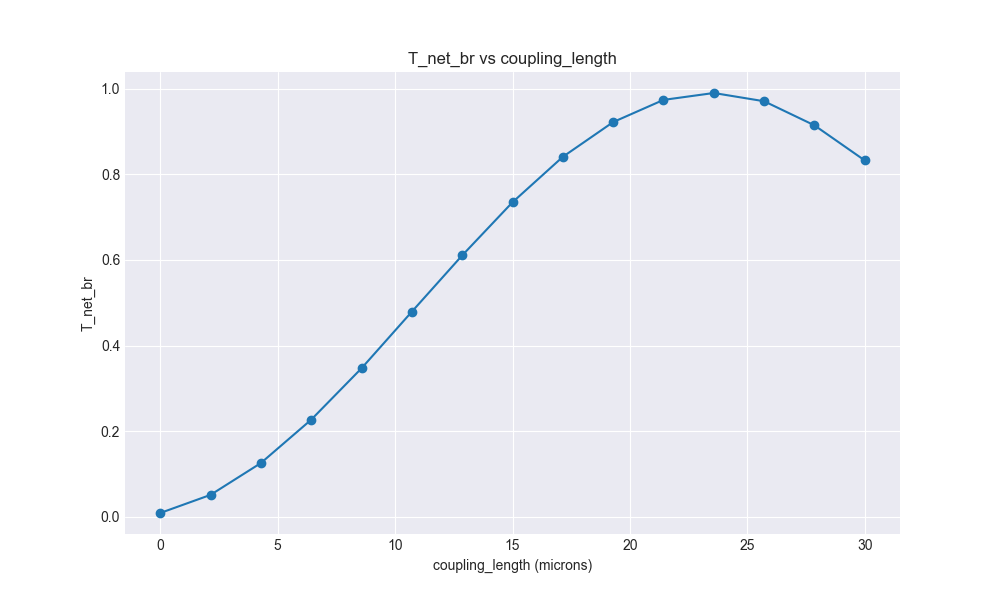
\includegraphics[width=0.8\textwidth]{task3/sweep_plots/sweep_idx_6_sweep__coupling_length=0_30_15_wg1_width=0.4_wg2_width=0.4_separation=0.15_center_wavelength=1.31_T_net_br_line.png}
  \caption{Cross-power transfer fraction at the coupled output port as a function of coupling length \(L\) for a fixed waveguide width of \SI{400}{\nm} and separation gap of \SI{150}{\nm} under input port TE\textsubscript{0} mode excitation at \SI{1310}{\nm}.}
  \label{fig:coupling_length_1310_w400}
\end{figure}

\subsection{Effect of waveguide width and separation gap}

It is not always so trivial to design a directional coupler that achieves the desired operation characteristics,
hence it is useful to explore the effect of the hyperparameters fixed before optimised over the coupling length \(L\),
namely the waveguide width and separation gap.

Figure~\ref{fig:2D_sweep_equal_wg_vs_sep} shows the power transfer fraction to the lower waveguide TE\textsubscript{0} mode monitor
as a function of the uniform waveguide width \(w\) swepth through \(w\in[0.1, 1.0]\,\unit{\um}\) and separation gap \(s\) swept through \(s\in[0.15, 0.5]\,\unit{\um}\) for a fixed coupling length of \SI{10}{\um} and input port TE\textsubscript{0} mode excitation at \SI{1550}{\nm}. For the majority of the parameter space, there is very weak coupling.
However, we observe a ridge of strong power transfer along the entire separation axis at a waveguide width of \(w=\SI{0.36}{\um}\),
with a peak at \(s=\SI{0.25}{\um}\). 

\begin{figure}[h!]
  \centering
  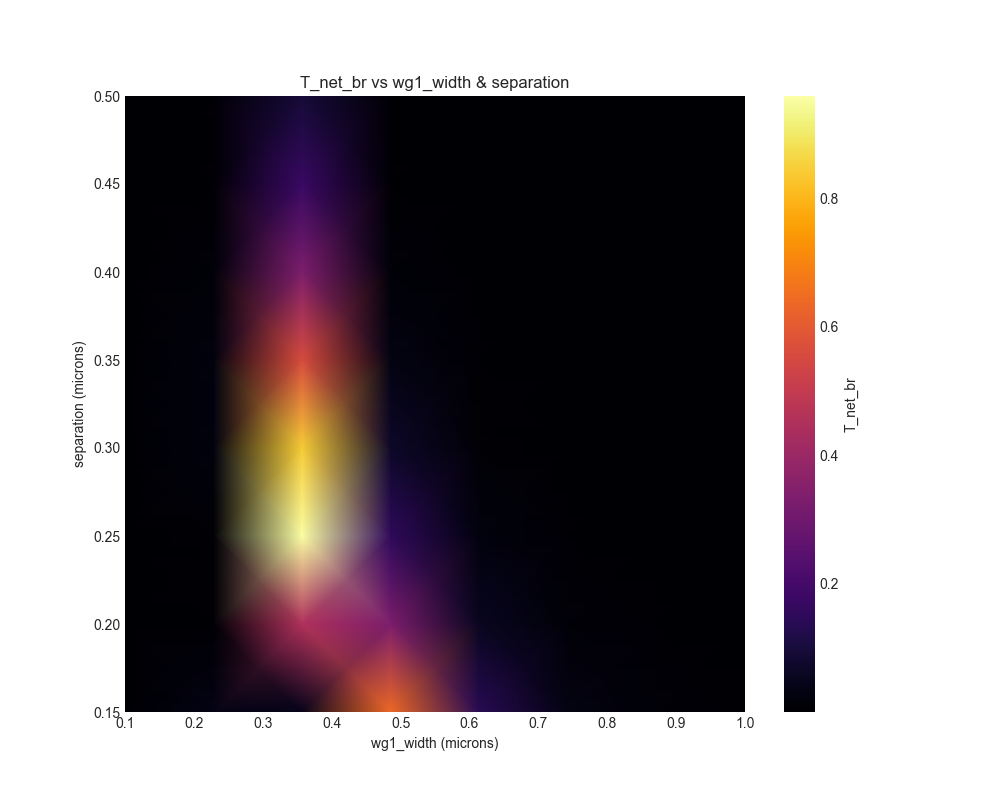
\includegraphics[width=0.8\textwidth]{task3/sweep_plots/sweep_idx_2_sweep__wg1_width=0.1_1_8,_wg2_width=0.1_1_8,_separation=0.15_0.5_8_(matched_widths)_T_net_br_heatmap.png}
  \caption{Cross-power transfer fraction at the coupled output port as a function of waveguide width \(w\) and separation gap \(s\) for a fixed coupling length of \SI{10}{\um} under input port TE\textsubscript{0} mode excitation at \SI{1550}{\nm}.}
  \label{fig:2D_sweep_equal_wg_vs_sep}
\end{figure}

\paragraph{Effect of waveguide width}
While a small waveguide width increases the evanescent overlap,
it also reduces the mode confinement and increases propagation losses,
hence there are very high bending-induced radiative losses for small waveguide widths.
Figure~\ref{fig:high_bend_loss} shows the power intensity distribution across the waveguide plane
for a waveguide width just before the ridge \(w=\SI{0.23}{\um}\) and at the optimal separation gap \(s=\SI{0.25}{\um}\).

From this it is clear that the mode is not well confined, and loses almost all of its power along the input port S-bend.

\begin{figure}[h!]
  \centering
  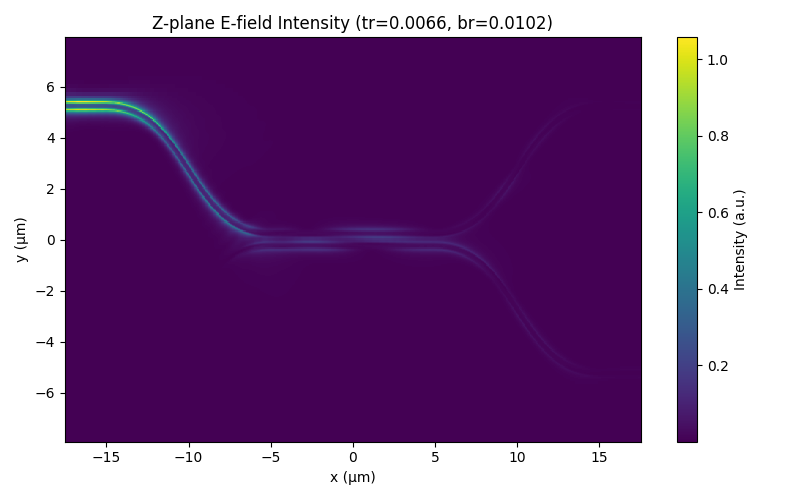
\includegraphics[width=0.8\textwidth]{task3/sim_0524_120625/z_plane_intensity.png}
  \caption{Power intensity distribution across the waveguide plane at the coupling length \(L=\SI{10}{\um}\) for a waveguide width of \(w=\SI{0.23}{\um}\) and separation gap of \(s=\SI{0.25}{\um}\) under input port TE\textsubscript{0} mode excitation at \SI{1550}{\nm}.}
  \label{fig:high_bend_loss}
\end{figure}

Very large waveguide widths, on the other hand, have much stronger mode confinement,
with a smaller evanescent tail, which reduces the coupling coefficient \(\kappa\) and thus the power transfer fraction.
(You could increase the coupling length \(L\) to compensate for this, in this plot it was held as constant.)
The optimal waveguide width is thus a balance between these two effects,
and the ridge of strong power transfer at \(w=\SI{0.36}{\um}\) is the result of this trade-off.

\paragraph{Effect of separation gap}

Now that we have established the optimal waveguide width,
in analysis of the separation gap, it may be more intuitive to fix the width at this optimum and consider effect of separation on the ridge profile,
which is shown in Figure~\ref{fig:coupled_power_ridge}.
At a large separation, the power transfer fraction decays exponentially,
but at a small separation, the power transfer fraction is also small and increases linearly with the separation gap.

The former can be rationalised by the fact that the evanescent tails of the modes in each waveguide overlap less and less as the separation gap increases.
However, the latter is less intuitive.
At very small separation,
the two-waveguide supermodes are heavily hybridized; effective indices split strongly,
resulting in a large coupling coefficient \(\kappa\). However, since the coupling length \(L\) is fixed,
the output phase of the power beating is not optimised for maximum cross-power transfer.
Indeed, Figure~\ref{fig:2D_sweep_equal_wg_vs_sep} show that, for very small separations,
the ridge of strong cross-power transfer moves diagonally towards larger waveguide widths.
Since increasing the waveguide width decreases the coupling coefficient \(\kappa\) by reducing the degree of hybridization,
these two effects cancel out, and the power transfer fraction remains optimised at the fixed coupling length \(L\).

\begin{figure}[h!]
  \centering
  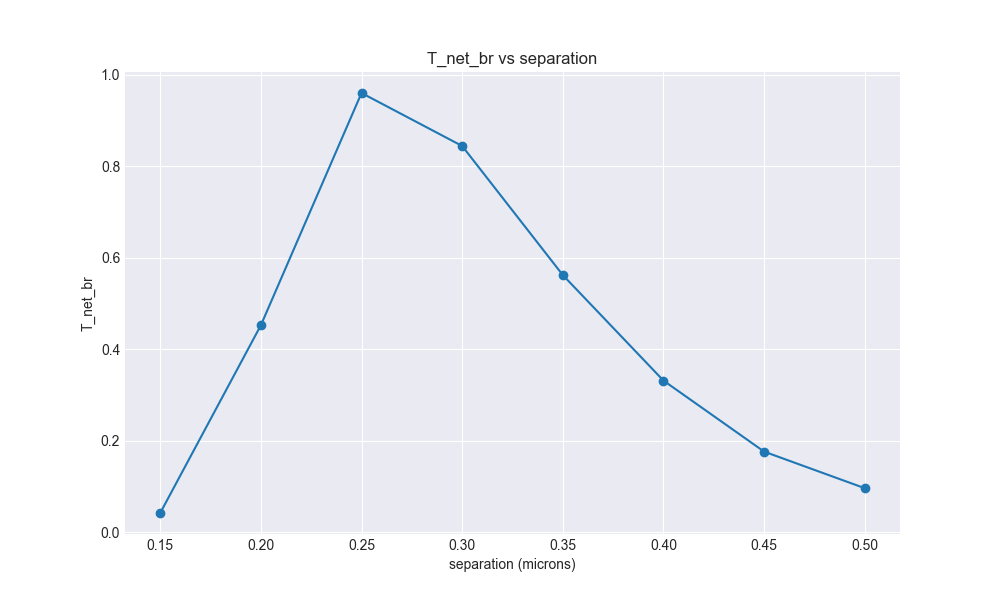
\includegraphics[width=0.8\textwidth]{task3/sweep_plots/sweep_idx_10_sweep__coupling_length=10_wg1_width=0.3571428571428572_wg2_width=0.3571428571428572_separation=0.15_0.5_8_center_wavelength=1.55_T_net_br_line.png}
  \caption{Cross-power transfer fraction at the coupled output port as a function of separation gap \(s\) for a fixed waveguide width of \(w=\SI{0.36}{\um}\) under input port TE\textsubscript{0} mode excitation at \SI{1550}{\nm}.}
  \label{fig:coupled_power_ridge}
\end{figure}

\subsection{Cross-order mode coupling}

Designing for coupling across modes of different orders is less trivial. 
For the TE\textsubscript{0}-TE\textsubscript{0} case we were able to rely on the fact that equal waveguide widths impose TE\textsubscript{0} phase matching across the separation gap,
but this is not the case for general cross-order mode coupling.

% I chose TE0-TE2
% TODO: show whether TE0-TE1 is possible, or if parity forbids it / requires lateral displacement of the 2nd waveguide

There is an additional step of design required to achieve cross-order mode coupling:
matching the effective indices of the two modes across the separation gap.

\paragraph{TE\textsubscript{0}-TE\textsubscript{2} coupling}
Let us consider the example of designing a directional coupler that transfers maximum power from the TE\textsubscript{0} mode of the upper waveguide to the TE\textsubscript{2} mode of the lower waveguide. 
Recall Figure~\ref{fig:te_neff} from the first interim report\autocite{ngSB4IntegratedPhotonics2025}.
This idealised planar case demonstrates that we expect that,
with the upper waveguide width fixed at \(w_1=\SI{0.4}{\um}\),
we expect it to be able to couple to the TE\textsubscript{2} mode of the lower waveguide when it is at a width \(1< w_2\leq 1.5\).

\begin{figure}[h!]
  \centering
  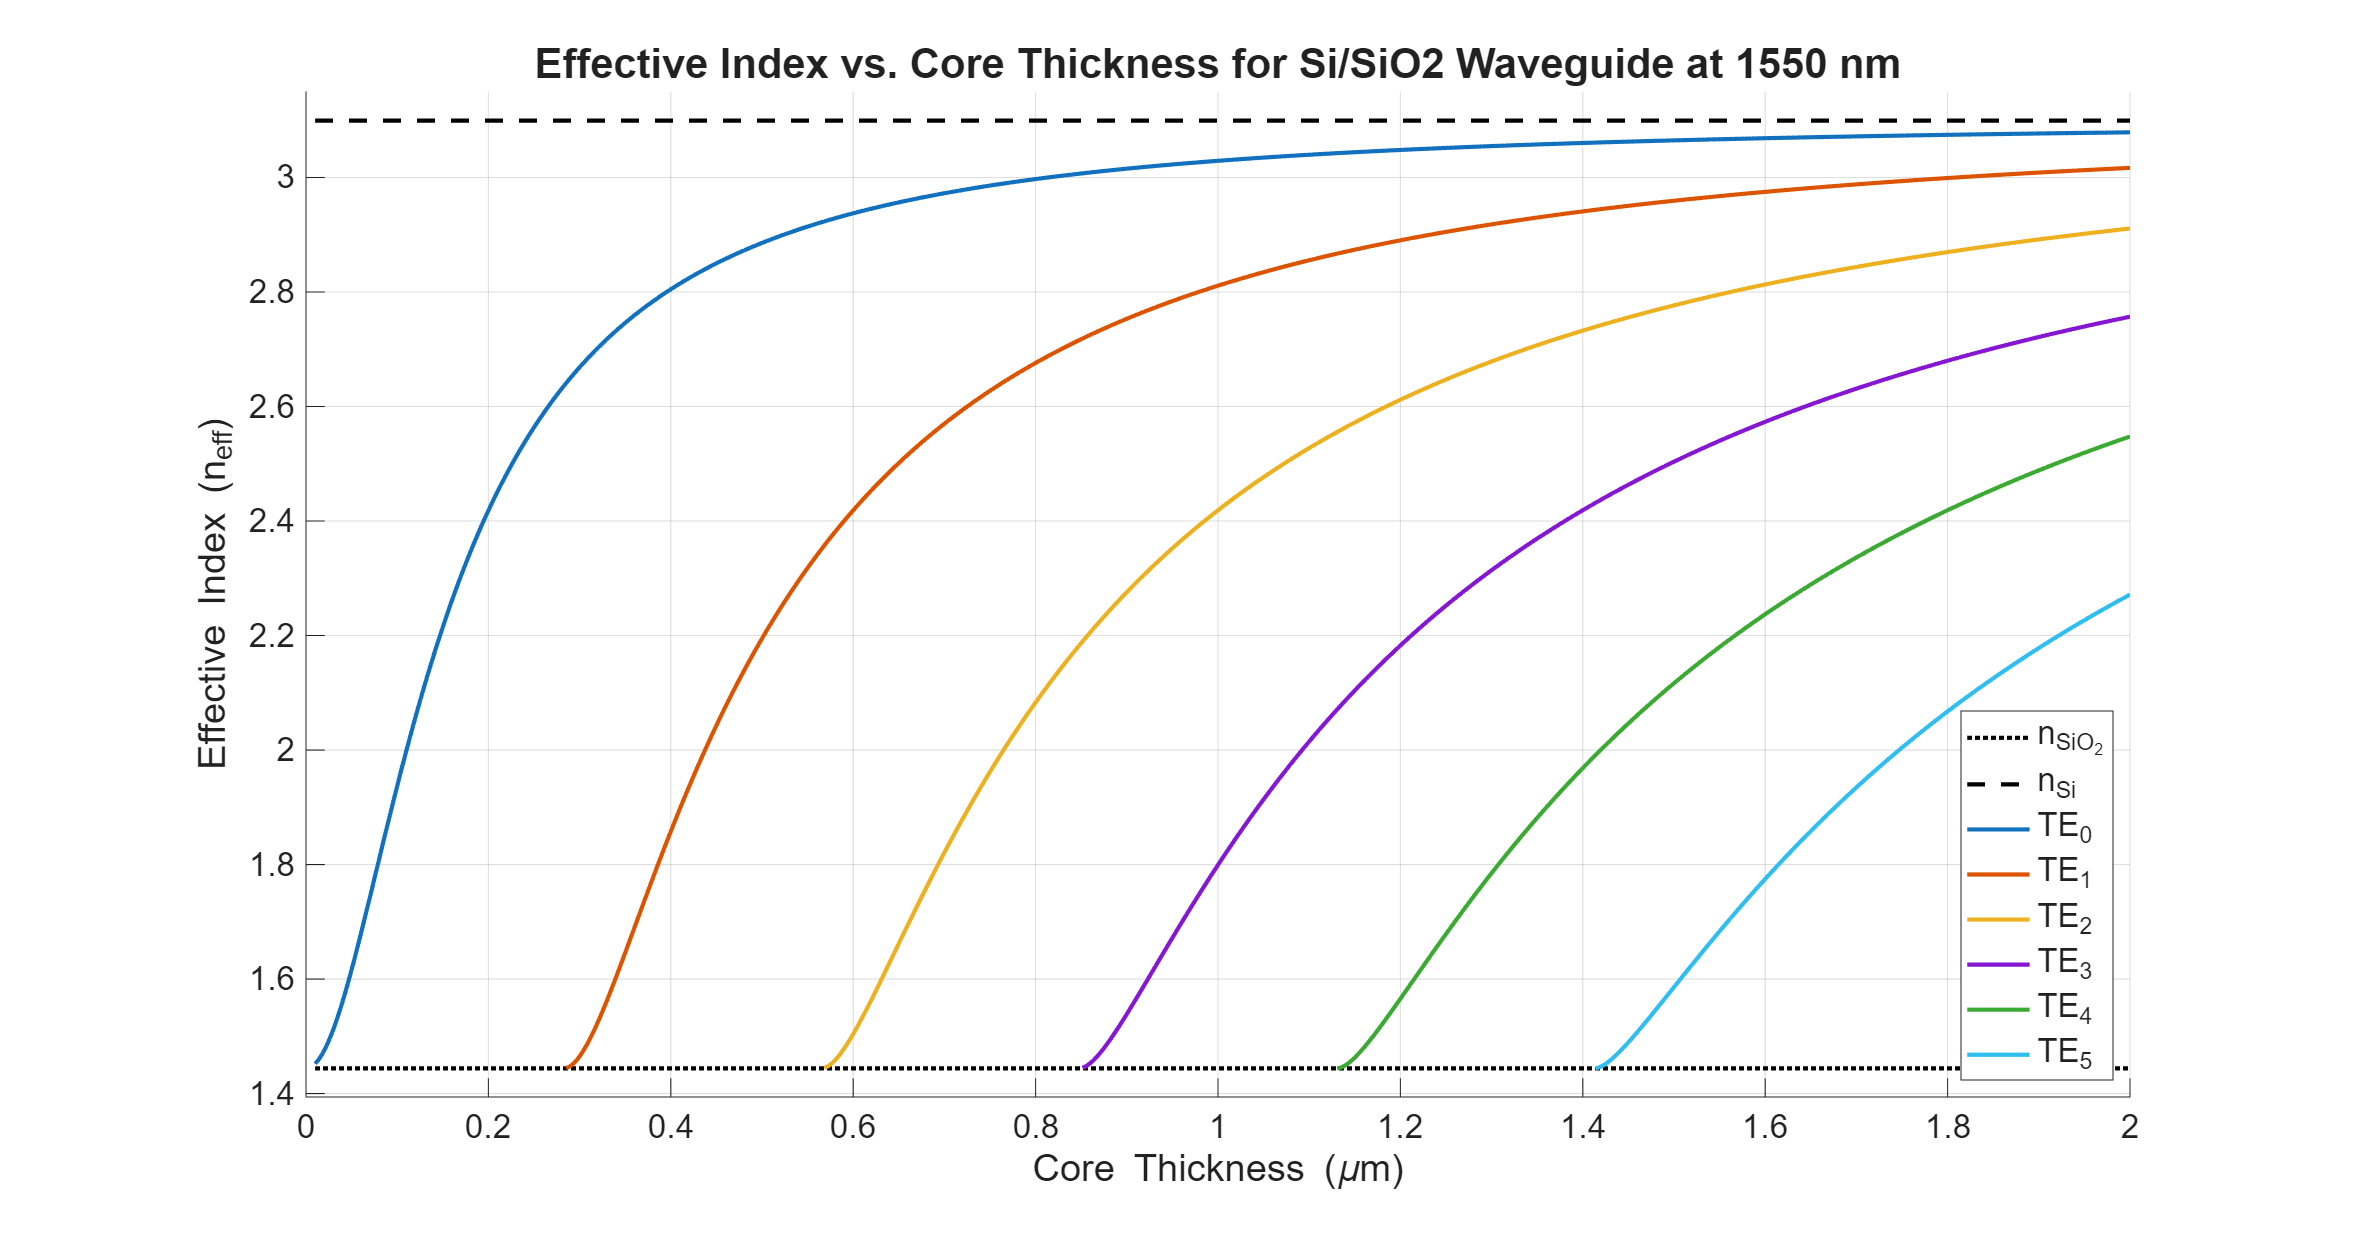
\includegraphics[width=0.8\textwidth]{task1/neff_vs_thickness_Si_SiO2_1550nm.png}
  \caption{Effective indices of TE\textsubscript{0}-TE\textsubscript{5} as a function of waveguide thickness.}
  \label{fig:te_neff}
\end{figure}

To avoid adding additional monitors to the simulation sweep,
it will suffice to use the upper output port TE\textsubscript{0} mode monitor as an inverse proxy for the lower output port TE\textsubscript{2} mode monitor.
One design strategy is to sweep both the lower waveguide width \(w_2\) through the range \(w_2\in(1,1.5]\,\unit{\um}\) and the coupling length \(L\in[10,40]\,\unit{\um}\) while keeping the separation gap fixed at \(s=\SI{0.15}{\um}\).
This produces the heatmap in Figure~\ref{fig:te0_te2_coupling_heatmap} of the power fraction received by the proxy TE\textsubscript{0} mode monitor on the upper waveguide.
\begin{figure}[h!]
  \centering
  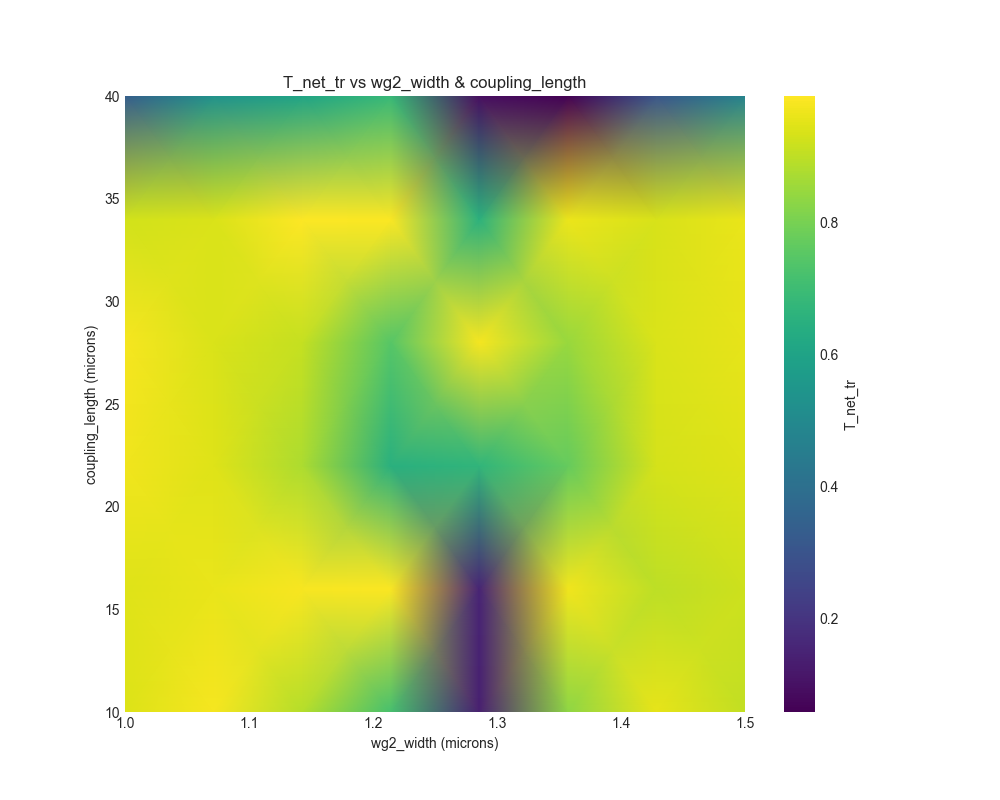
\includegraphics[width=0.8\textwidth]{task3/sweep_plots/sweep_idx_7_sweep__coupling_length=10_40_6_wg1_width=0.4_wg2_width=1_1.5_8_separation=0.15_center_wavelength=1.55_T_net_tr_heatmap.png}
  \caption{Cross-power transfer fraction at the upper waveguide TE\textsubscript{0} mode monitor as a function of lower waveguide width \(w_2\) and coupling length \(L\) for a fixed upper waveguide width of \(w_1=\SI{0.4}{\um}\) and separation gap of \(s=\SI{0.15}{\um}\) under input port TE\textsubscript{0} mode excitation at \SI{1550}{\nm}.}
  \label{fig:te0_te2_coupling_heatmap}
\end{figure}

Clearly, we have a sinusoidal ridge of recorded power transfer
along the coupling length axis,
at a waveguide width of \(w_2=\SI{1.28}{\um}\).
Fixing that width and looking along at ridge results in Figure~\ref{fig:te0_te2_coupling_length}, showing the optimum coupling length \(L\) for maximum power transfer to the TE\textsubscript{2} mode of the lower waveguide 
to be \(\hat{L}\approx\SI{13}{\um}\). Figure~\ref{fig:cross_mode_power_distribution} shows the power intensity distribution across the waveguide plane at this coupling length,
with the TE\textsubscript{0} mode monitor on the upper waveguide registering a power transfer fraction of \(0.0182\) and the TE\textsubscript{2} mode monitor on the lower waveguide registering a power transfer fraction of \(0.9235\). This means the TE\textsubscript{2} mode is excited to \(98.1\%\) of the total power fraction it shares with the TE\textsubscript{0} mode at the input port of the upper waveguide. There is some launched power unaccounted for, but that can be assigned to modal leakage.

This is the directional coupler shown originally in Figure~\ref{fig:s_bend_coupler}.

\begin{figure}[h!]
  \centering
  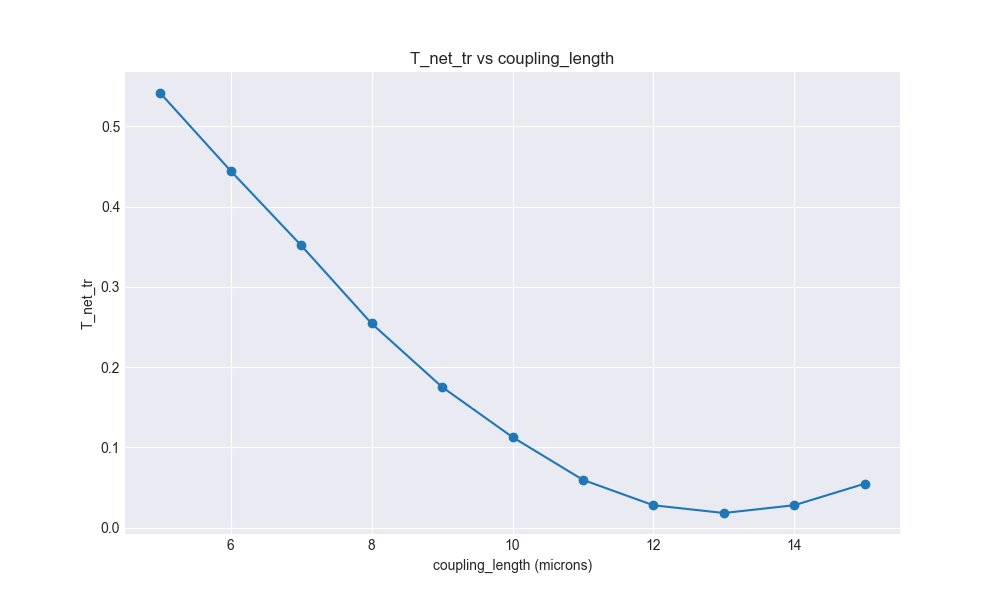
\includegraphics[width=0.8\textwidth]{task3/sweep_plots/sweep_idx_8_sweep__coupling_length=5_15_11_wg1_width=0.4_wg2_width=1.28_separation=0.15_center_wavelength=1.55_T_net_tr_line.png}
  \caption{Power transfer fraction at the upper waveguide TE\textsubscript{0} mode monitor as a function of coupling length \(L\) for a fixed upper waveguide width of \(w_1=\SI{0.4}{\um}\), lower waveguide width of \(w_2=\SI{1.28}{\um}\), and separation gap of \(s=\SI{0.15}{\um}\) under input port TE\textsubscript{0} mode excitation at \SI{1550}{\nm}.}
  \label{fig:te0_te2_coupling_length}
\end{figure}
\begin{figure}[h!]
  \centering
  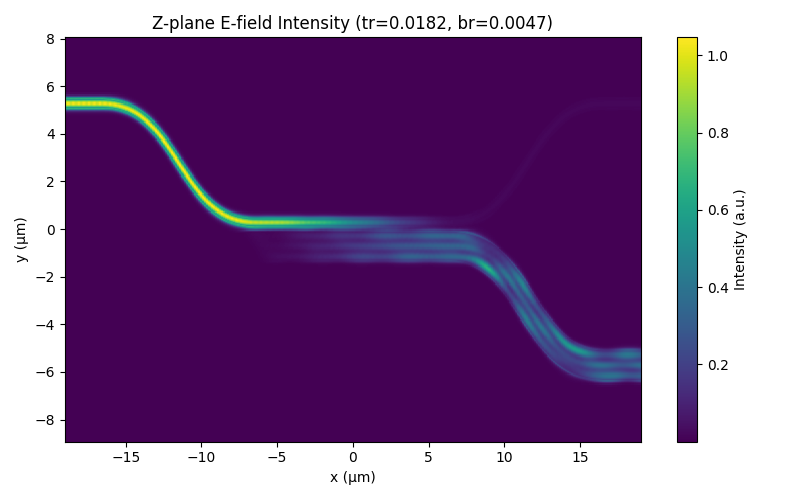
\includegraphics[width=0.8\textwidth]{task3/sim_1521_130625/z_plane_intensity.png}
  \caption{Power intensity distribution across the waveguide plane at the coupling length \(L=\hat{L}\approx\SI{13}{\um}\) for a fixed upper waveguide width of \(w_1=\SI{0.4}{\um}\), lower waveguide width of \(w_2=\SI{1.28}{\um}\), and separation gap of \(s=\SI{0.15}{\um}\) under input port TE\textsubscript{0} mode excitation at \SI{1550}{\nm}.}
  \label{fig:cross_mode_power_distribution}
\end{figure}



\section{Other contributions}


\section{Conclusion}


\printbibliography
\end{document}